\chapter{Electrochemical impedance spectroscopy and equivalent circuit model for AA alkaline batteries\label{ch:eis}}

Our results in Fig.~\ref{fig:EIS} agree with previous impedance spectroscopy experiments on alkaline LR6-type cells.~\cite{wang,root} In the Nyquist plots, high reactance (Z") and resistance (Z') are visible in the as-received cell, with a two order of magnitude drop in both following 10\% discharge of the cell. A maximum in solution resistance occurs at 50\% SOC. Reactance remains constant. Our tests of our system show that it can be modeled with a standard Randles circuit, modified by the addition of a second phase with separate charge-transfer and double-layer capacitance impedance values. This model is shown in Fig.~\ref{fig:EIS}a. Over time, the ohmic impedance of the system, typically dominated by the ionic impedance of the electrolyte, stays roughly constant with state of charge (SOC), up until 50\% SOC, when a significant spike in ohmic impedance occurs. This increase correlates with the leveling of the coefficient of restitution changes caused by the transition between the formation of Type I ZnO to Type II ZnO. The double-layer capacitance of both phases present decreases with decreasing state-of-charge. This suggests that there is a continuous decrease in the total surface area of the available Zn anode with cycling, which correlates well with the phase transformation from Zn to ZnO, as ZnO is less dense than Zn. This is in strong agreement with Haibel, Manke and Gallaway.~\cite{haibel,Manke2007-yj,gallaway}  What we see is a complex mix within the impedance data, where increasing impedance throughout the entire discharge is attributed to 1) loss of solvent (consumption of water) in the protonation of \ce{MnO_2} and the oxidation of Zn, 2) ZnO formation which passivates and blocks the Zn surface, and 3) increasing concentration of alkaline salts in the remaining water which decreases the conductivity of the electrolyte above.~\cite{linden}

\begin{figure}[htb]
  \centering
    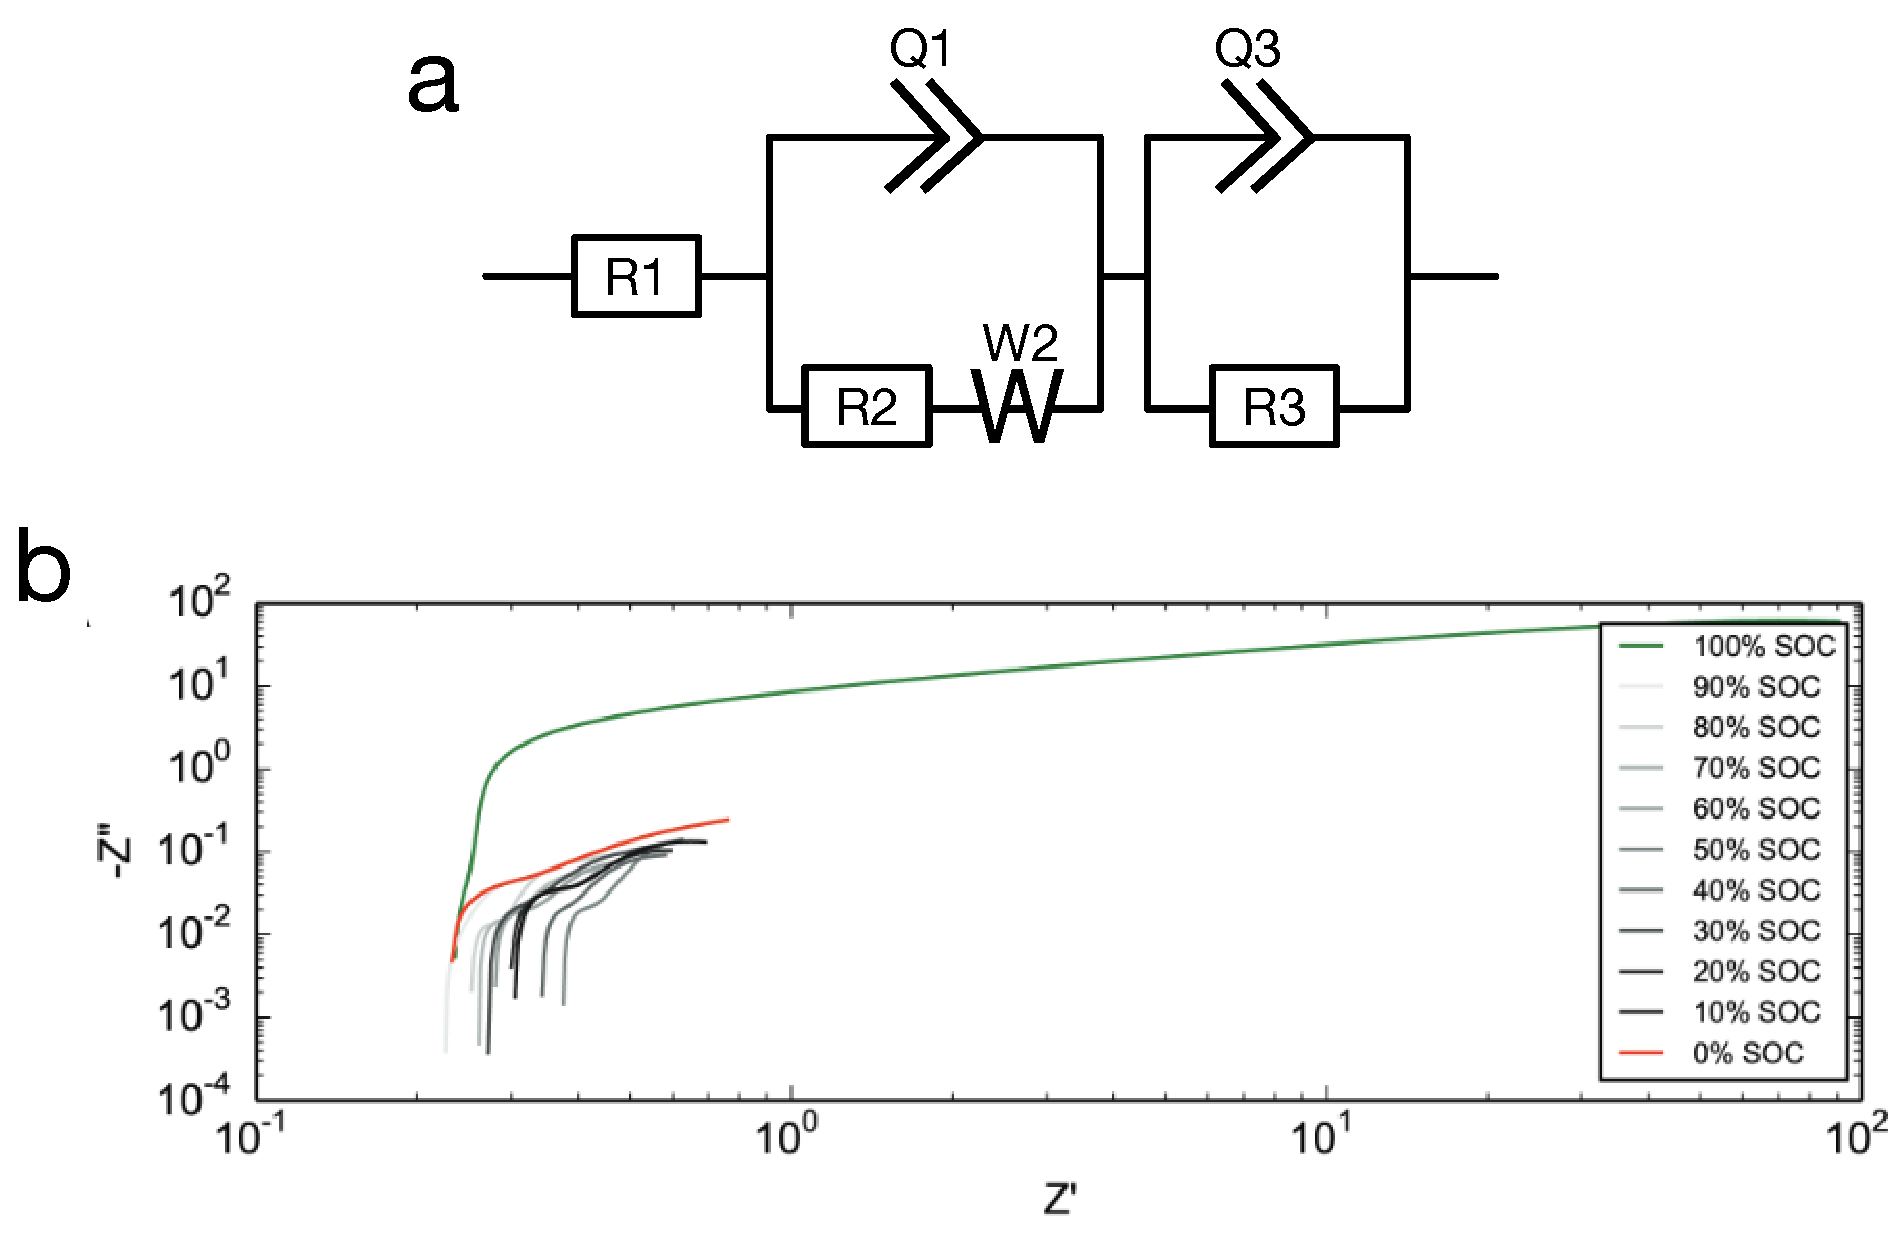
\includegraphics[width=\textwidth]{ch-appendices/images/Supp5.pdf}
    \caption[Equivalent circuit model and Nyquist plot for \textit{in situ} EIS performed on a AA alkaline battery]{a) Circuit diagram of EIS model used; b) Nyquist impedance plot for a representative cell, measured from as-received (green) to fully-discharged (red). Scans performed from 100 mHz to 100 kHz.}
    \label{fig:EIS}
\end{figure}